

%%% use twocolumn and 10pt options with the asme2e format
\documentclass[twocolumn,10pt]{asme2e}
\usepackage{graphicx}
\usepackage{graphics}
\usepackage{amsmath}
%\usepackage{amsthm}
\usepackage{amsfonts}

\newtheorem{assumption}{Assumption}
\newtheorem{definition}{Definition}
\newtheorem{theorem}{Theorem}
\newtheorem{lemma}{Lemma}
%\newtheorem{example}{Example}

\newcommand{\todo}[1]{\vspace{5 mm}\par \noindent
\marginpar{\textsc{Todo}}
\framebox{\begin{minipage}[c]{0.40 \textwidth}
\tt \flushleft #1 \end{minipage}}\vspace{5 mm}\par}

\newtheorem{example_base}{Example}
\newenvironment{example}{\begin{example_base}}
   {\hspace{\stretch{1}}$\lozenge$\end{example_base}}

\graphicspath{{figures/}}
\DeclareMathOperator{\erf}{erf}
\DeclareMathOperator{\prob}{Prob}

%% The class has several options
%  onecolumn/twocolumn - format for one or two columns per page
%  10pt/11pt/12pt - use 10, 11, or 12 point font
%  oneside/twoside - format for oneside/twosided printing
%  final/draft - format for final/draft copy
%  cleanfoot - take out copyright info in footer leave page number
%  cleanhead - take out the conference banner on the title page
%  titlepage/notitlepage - put in titlepage or leave out titlepage
%
%% The default is oneside, onecolumn, 10pt, final

%%% Replace here with information related to your conference
\confshortname{DSCC 2008} \conffullname{ASME 2008 Dynamic
Systems and Control Conference} \confdate{20-22}
\confmonth{October} \confyear{2008} \confcity{Ann Arbor,
Michigan} \confcountry{USA}

%%% Replace DETC2005-12345 with the number supplied to you
%%% by ASME for your paper.
\papernum{DSCC2008-12345}

\title{Numerical Evidence for Cutoffs in Chaotic Microfluidic Mixing}

%%% first author
\author{Tzu-Chen Liang
    \affiliation{
    Department of Aeronautics and Astronautics\\
    Stanford University\\
    Stanford, California 94305\\
    Email: tzuchen@stanford.edu
    }
}

%%% second author
%%% remove the following entry for single author papers
%%% add more entries for additional authors
\author{Matthew West 
    \affiliation{
    Department of Mechanical Science and Engineering\\
    University of Illinois at Urbana-Champaign\\
    Urbana, Illinois, 61801\\
    Email: mwest@illinois.edu
    }
}

\begin{document}

\maketitle
%%%%%%%%%%%%%%%%%%%%%%%%%%%%%%%%%%%%%%%%%%%%%%%%%%%%%%%%%%%%%%%%%%%%%%
%%%%%%%%%%%%%%%%%%%%%%%%%%%%%%%%%%%%%%%%%%%%%%%%%%%%%%%%%%%%%%%%%%%%%%
\begin{abstract}
%need to be less than 150 words!
Chaotic mixing strategies produce high mixing rates in microfluidic
channels and other applications. In prior numerical and experimental
work the variance of a tracer field in a chaotic mixer has been
observed to decay rapidly after an initial slower transient. We relate
this to the cutoff phenomenon observed in finite Markov chains and
provide numerical evidence to suggest that chaotic mixing indeed
exhibits cutoff. We provide results for a herringbone passive
microfluidic mixer and the Standard Map.
\end{abstract}

%%%%%%%%%%%%%%%%%%%%%%%%%%%%%%%%%%%%%%%%%%%%%%%%%%%%%%%%%%%%%%%%%%%%%%
%\begin{nomenclature}
%\entry{A}{You may include nomenclature here.}
%\entry{$\alpha$}{There are two arguments for each entry of
%the nomemclature environment, the symbol and the
%definition.}
%\end{nomenclature}

%The spacing between abstract and the text heading is two
%line spaces.  The primary text heading is  boldface in all
%capitals, flushed left with the left margin.  The spacing
%between the  text and the heading is also two line spaces.

%%%%%%%%%%%%%%%%%%%%%%%%%%%%%%%%%%%%%%%%%%%%%%%%%%%%%%%%%%%%%%%%%%%%%%
\section*{INTRODUCTION}

The question of how chaotic advection mixes a passive scalar function
has attracted much research effort in recent years~
\cite{Ottino2004}. The main issues in this field are: how to measure
the thoroughness of the mixing, how the mixing process changes
qualitatively and quantitatively when the diffusion is close to zero,
and how to enhance the overall mixing process by designing the map
which produces chaotic advection. Unfortunately, we have only partial
understanding for most of these topics. In spite of the fact that the
detailed mechanism of mixing is unclear, non-trivial mixing processes
have been observed in experiments~\cite{Voth2002} and
can be simulated by large-scale computations~\cite{Tsang2005}. 




A widely observed phenomenon in the chaotic mixing process when small
diffusion exists is the two or three-stage transition~
\cite{Thiffeault2003-13, Fereday2002, Mezic2005}. The
map does not mix the scalar function with a constant rate in
general. When the variance of the scalar function is measured during
the mixing process, one can in general observe a relatively flat decay
initially, followed by a super-exponential change, and then finally it
tends to an exponential decay. We are interested in when these
transitions happen, why they happen, and how to predict the slope of
the exponential region. A good review and physical interpretation can
be found in~\cite{Thiffeault2004}.

Thiffeault and Childress~\cite{Thiffeault2003-13} study these
properties for a modified Arnold's cat map. Analytical formulas are
given to predict the transitions as well as the slopes. Because the
linear part of this map has an eigenvalue 2.618, which stretches very fast, 
and the chaotic part is relatively small, the three phases are
separated clearly. The same analytical procedure cannot be applied to,
for example, the Standard Map, although the only difference between the
Standard Map and the modified Arnold's cat map is in the linear part.

As for the exponential decay part, there is still debate about whether
the decay rate goes to zero in the zero diffusivity limit or whether
it tends to a constant independent of the diffusion~
\cite{Thiffeault2004, Tsang2005}. Theoretical analysis shows both of
these possibilities can occur for different chaotic flows
~\cite{Haynes2005}.

Difficulties typically arise in studying the above problems
numerically, because the small diffusion usually means that fine grids
are required in the solution of the advection-diffusion equation or
the simulation of the map. Some studies and numerical results conclude
that a proportional relation exists between the stationary decay rate
and the diffusion~\cite{Cerbelli2003}. However, this is only true for
certain diffusion ranges.

Our goal in this paper is to relate the chaotic mixing process to the
well-known cutoff phenomenon in finite Markov Chain studies
(see\cite{Diaconis2005} and references therein). We begin with a
numerical simulation of a chaotic mixing channel, measuring mixing of
two colored liquids by the color variance of channel
cross-sections. The simulation shows that when we increase the
P\'{e}clet number, the mixing trajectory presents a cutoff. The
underlying physical mechanism is then explained using advection of a
sinusoidal function under the Baker's Map. To support the chaotic
mixing channel example, a very high resolution numerical simulation of
the Standard Map is then presented to show that in the near-zero
diffusion limit it does present a cutoff.

%%%%%%%%%%%%%%%%%%%%%%%%%%%%%%%%%%%%%%%%%%%%%%%%%%%%%%%%%%%%%%%%%%%%%%
\section*{BACKGROUND}%%%%%%%%%%%%%%%%%%%%%%%%%%%%%%%%%%%%%%%%%%%%%%%%%
%%%%%%%%%%%%%%%%%%%%%%%%%%%%%%%%%%%%%%%%%%%%%%%%%%%%%%%%%%%%%%%%%%%%%%

%%%%%%%%%%%%%%%%%%%%%%%%%%%%%%%%%%%%%%%%%%%%%%%%%%%%%%%%%%
\subsection*{The measure space and operators}
%%%%%%%%%%%%%%%%%%%%%%%%%%%%%%%%%%%%%%%%%%%%%%%%%%%%%%%%%%

We work on the probability space $(X,\mathcal{A},\mu)$ for $X$ a
subset of $\mathbb{R}^n$. We take $S: X \to X$ to be a transformation
(or map) that is non-singular and measurable. We choose $\mu$ to be
the Borel measure. In the measure space $(X,\mathcal{A},\mu)$ we
define the following operators.


\begin{definition} \textbf{(Perron-Frobenius operator)}
The Perron-Frobenius operator $P:L^1(X) \to L^1(X)$ associated with
$S$ satisfies
\begin{equation}
  \int_A (P \omega)(x)\mu(dx) = \int_{S^{-1}(A)} \omega(x)\mu(dx)
\end{equation}
for every $\omega \in L^1(X)$ and $A \in \mathcal{A}$.
\end{definition}
The Perron-Frobenius operator is linear. Because of our choice of
measure space, the Perron-Frobenius operator can be interpreted as a
map that evolves probability density functions. Also, suppose that
$\bar{\omega}$ is an invariant measure of $S$, so that
$\bar{\omega}(S^{-1}(A)) = \bar{\omega}(A)$ for all $A \in
\mathcal{A}$.  Then we have $P \bar{\omega} = \bar{\omega}$ (omitting
$x$).

\begin{definition} \textbf{(Koopman operator)}
Let $f \in L^\infty(X)$. The operator $U:L^{\infty}(X) \to
L^{\infty}(X)$ defined by $Uf(x) = f(S(x))$ is called the Koopman
operator associated with $S$.
\end{definition}
The Koopman operator is adjoint to Perron-Frobenius operator, which we
write as $U = P^*$.

In the measure space $(X,\mathcal{A},\mu)$, where $\mu$ is the Borel
measure, let $P_S$ and $U_S$ be the Perron-Frobenius and the Koopman
operators of an invertible map $S$. We have the following relations:
\vspace{0.15cm}
\begin{center}
\begin{tabular}{l|ll}
\label{PUtable}
& forward in time
& backward in time
\\
\hline
probability density
& $P_S$
& $P_{S^{-1}}$
\\
scalar function
& $ U_{S^{-1}} = P_{S^{-1}}^* $
& $ U_S = P_S^*  $
\end{tabular}
\end{center}
\vspace{0.15cm} Our goal is to simulate how a scalar function is
advected by a chaotic map forward in time. From the above table, it is
clear we should use the operator $U_{S^{-1}}$. For a given initial
function $f^0(x)$, one has, $f^{k+1} = U_{S^{-1}} f^k$, for all $k$.

%%%%%%%%%%%%%%%%%%%%%%%%%%%%%%%%%%%%%%%%%%%%%%%%%%%%%%%%%%
\subsection*{Numerical Strategy}
%%%%%%%%%%%%%%%%%%%%%%%%%%%%%%%%%%%%%%%%%%%%%%%%%%%%%%%%%%

Numerically, an approximation of $U_{S^{-1}}$ is used. For a map $S: X \to X$, we discretize $X$ into regular square grids with size $h$. The grids are numbered as $a_1,a_2,.., a_{n}$. We first define a map (an observer) $g_n: f(x) \mapsto
f_n $ such that
\begin{eqnarray} 
  (f_n)_i = (g_n(f(x)))_i = \int_{a_i} f(x) \mu(dx) \mbox{, for }i = 1
  \mbox{ to } n.
\end{eqnarray}
This $g_n$ maps the scalar function we are interested into a finite
length vector in $\mathbb{R}^n$, and thus we only need a linear
operator $B_n:\mathbb{R}^n \to \mathbb{R}^n$ to approximate
$U_{S^{-1}}$, and thus to evolve the function in the reduced space
$\mathbb{R}^n$. The $B_n$ we use in our numerical simulation is
obtained in a very simple way: let $\mathbf{x}_i =(x_{1i},x_{2i})$ be
the center of grid $a_i$, then define a matrix $B_n$ as,
 \begin{eqnarray}
 \label{finegridmethod}
 (B_n)_{ij} = \begin{cases}
   \frac{1}{4} &\mbox{, if } S(x_{1j}\pm \frac{h}{2},x_{2j}\pm \frac{h}{2}) \in a_i, \\
   0           &\mbox{, otherwise}. \\
 \end{cases}
 \end{eqnarray}
The matrix $B_n$ has only $4$ non-zeros in each row. For a given
$f^0$, we can thus approximate the evolution by $f_n^{k+1} = B_n
f_n^k$.

This approach is similar to the lattice
method~\cite{Pierrehumbert2000, Tsang2005}. We stress that there exist
better approximations of $U_{S^{-1}}$ which minimize the difference
between $f_n^k$ and $g_n(f^k)$~\cite{Froyland2001} by applying optimal
model reduction. However, our simple numerical strategy allows us to
go up to very large $n$ and to simulate the system with very small
numerical diffusion. During the simulation, the matrix $B_n$ is never
explicitly formed and we need only store a length $n$ state vector,
ensuring system evolution has cost of order $n$.


Using the above numerical strategy, we can evolve a function or a
probability distribution by the map with some small numerical
diffusion. The effect of numerical diffusion is similar to physical
diffusion on large scales, but their behavior can be quite different
on small scales. To simulate the physical diffusion correctly, we need
to simulate the map with higher resolution with some additional
physical diffusion added. The additional diffusion can be added in
either spatial or frequency domains. In the spatial domain, we adopt
the method of adding a smoothing step used in~\cite{Tsang2005},
 \begin{equation}
 \label{smoothingstep}
   f^{k+1}_{(p,q)} = \sum_{|r|,|s|\le 2}C_{|r|}C_{|s|}f^{k}_{(p,q)}
 \end{equation}
with $C_0=1/8, C_1=1/4$, and $C_2=3/16$ and $(p,q)$ is the 2-D index
of a grid. This creates a large scale diffusion $D \approx h^2$, which
is several times larger than the numerical
diffusion~\cite{Tsang2005}. We use a smoothing operator $M_n$ and
$f^{k+1} = M_n(f^{k})$ to denote the above smoothing step and define
$\bar{B}_n = M_n \circ B_n$.

Alternatively, in frequency domain a two dimensional FFT/IFFT with a
wave-number dependent scaling can be applied to simulate physical
diffusion. This procedure is denoted by an operator $F_n$, $f^{k+1} =
F_n(f^{k})$ and $\hat{B}_n = F_n \circ B_n$. Note that the FFT/IFFT
scheme is much more expensive when $n$ is large.


%%%%%%%%%%%%%%%%%%%%%%%%%%%%%%%%%%%%%%%%%%%%%%%%%%%%%%%%%%
\subsection*{Notion of a cutoff}
%%%%%%%%%%%%%%%%%%%%%%%%%%%%%%%%%%%%%%%%%%%%%%%%%%%%%%%%%%
In some Markov Chains, certain probability distributions converge to
an equilibrium via a sharp transition, which becomes sharper for
larger chains. This phenomenon is referred to as \emph{cutoff} in the
finite Markov chain literature~\cite{Diaconis2005}. Here we
extend the usual definition slightly to accommodate converge to
non-zero distance values.

To any finite set $\Omega$ and any pair of probability measures
$\omega$, $\bar{\omega}$ on $\Omega$ we associate a real number
$d(\omega,\bar{\omega})$ such that
\begin{subequations}
\label{eqn:defn_d}
\begin{align}
d(\omega,\bar{\omega}) &\in [0,1] \\
d(\omega,\bar{\omega}) &= 0 \text{ if and only if } \bar{\omega}=\omega \\
\max_{\Omega,\omega,\bar{\omega}} d(\omega,\bar{\omega}) &= M_d.
\end{align}
\end{subequations}
Note that $d$ need not satisfy the triangle inequality and so is not a
metric.

Consider a sequence of finite probability spaces $(\Omega_n)$ for $n =
1,2,\ldots$. We think of $n$ as the size of the space. Each space is
equipped with a probability measure $\bar{\omega}_n$ which we think of
as the unique invariant measure of a Markov chain on $\Omega_n$. For
each $n$ we now take a sequence of probability measures $\omega_n^k$
for $k = 0,1,2,\ldots$ such that
$\lim_{k \rightarrow \infty} d(\omega_n,\bar{\omega}_n)=0$.
The $\omega_n^k$ should be thought of as an initial condition
$\omega_n^0$ and then iterates of the distribution under the
evolution of a Markov chain.
\begin{definition}[Cutoff]
\label{cutoffdefinitionn}
Take a family $(\Omega_n,\bar{\omega}_n,
(\omega^k_n)_{k=0}^{\infty})_{n=1}^{\infty}$ of finite probability
spaces $\Omega_n$ and probability measures $\bar{\omega}_n$ and
$\omega_n^k$. This family presents a $d$-cutoff if there exists a
sequence $(t_n)_{n=1}^{\infty}$ of positive reals such that, for any
$\epsilon \in (0,1)$,
\begin{subequations}
  \label{eqn:defn_cutoff}
  \begin{align}
    \label{eqn:defn_cutoff_1}
    \lim_{n \rightarrow \infty}d(\omega^{k_n}_n,\bar{\omega}_n) &= m \text{ if }
    k_n > (1+\epsilon)t_n \\
    \lim_{n \rightarrow \infty}d(\omega^{k_n}_n,\bar{\omega}_n) &= M \text{ if }
    k_n < (1-\epsilon)t_n
  \end{align}
\end{subequations}
\end{definition}



This definition is taken from~\cite{Diaconis2005} with the change that
$m$ and $M$ are $0$ and $M_d$ in the original. The reason for this
modification will be clear when we present the results of Standard Map
simulation.

The definition of cutoff implies that the change of
$d(\omega_n^k,\bar{\omega}_n)$ from $M$ to $m$ happens ever more
rapidly as $n$ increases, but only in relation to the cutoff times
$t_n$. We can think of this as rescaling the each trajectory
$(\omega_n^k)_{k=0}^{\infty}$ in time by $t_n$ and seeing cutoff as
the limit of these rescaled trajectories to a step function. We give an example of cutoff phenomenon:

\begin{example} \textbf{Random walk on an $n$-dimensional hypercube} (Diaconis~\cite{Diaconis1990})
A particle starts at the origin and moves to one of its nearest
neighbors (or stays fixed) with equal probability at each step. The
problem can be formulated as a Markov Chain with $2^n$ states and the
invariant distribution $\bar{\omega}$ is uniform. The $|\omega^k_n -
\bar{\omega} |_{TV}$ (Total Variation Distance) versus iteration plot
with different $n$ is shown in Figure~\ref{rdwalk}.
\begin{figure}
       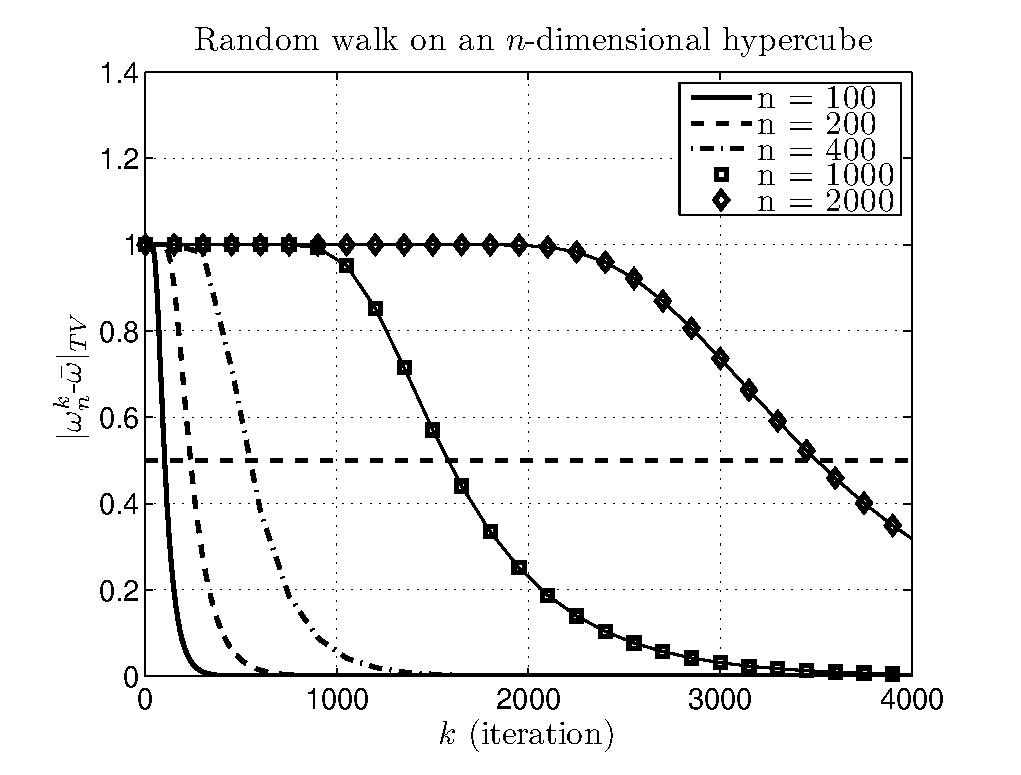
\includegraphics[width=0.45\textwidth,trim=1cm 0cm 0cm 0cm]{rdwalk}
       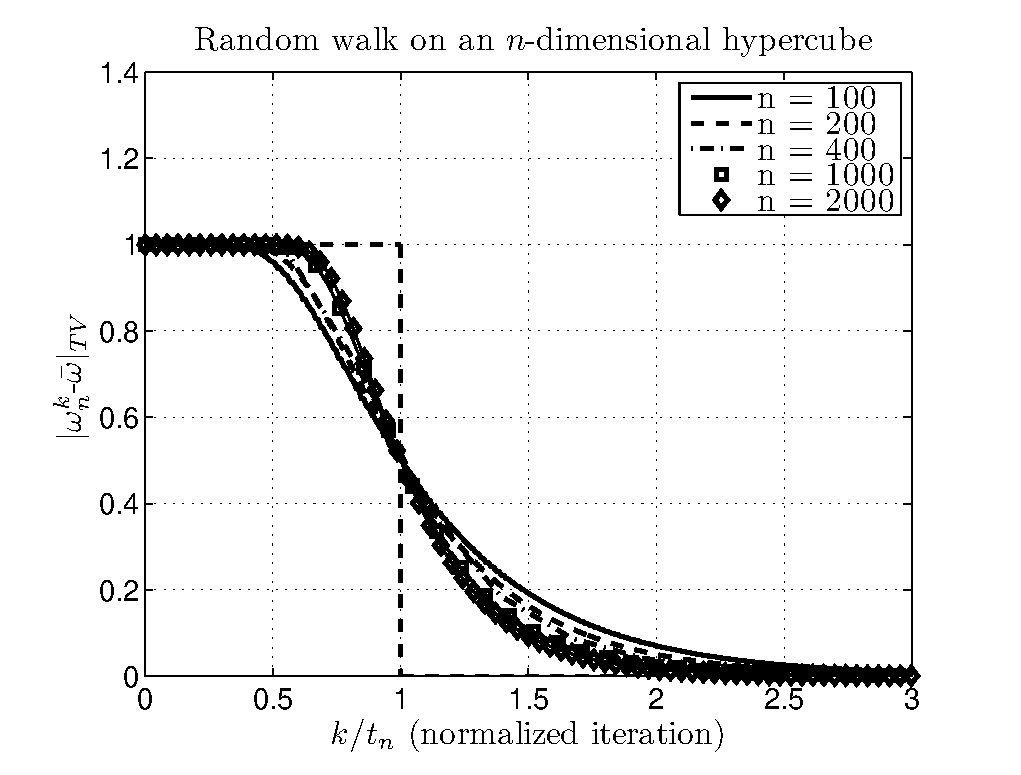
\includegraphics[width=0.45\textwidth,trim=1cm 0cm 0cm 0cm]{rdwalkn} 
       \caption{\label{rdwalk} THE UPPER FIGURE SHOWS THE EVOLUTION OF
         A MEASURE TO THE INVARIANT MEASURE FOR A RANDOM WALK ON AN
         $n$-DIMENSIONAL HYPERCUBE. WHEN $n$ INCREASES, THE DISTANCE
         STAYS CLOSE TO $1$ FOR LONGER BEFORE IT DROPS TO ZERO. THE
         BOTTOM FIGURE HAS TRAJECTORIES RESCALED IN $k$ TO SHOW CUTOFF
         AS A LIMIT TO A STEP FUNCTION.}
\end{figure}
\end{example}


\subsection*{How to recognize a cutoff?}
To prove the existence of a cutoff is in general very hard, relying on
special features of the sequence of systems. In this article we merely
provide numerical evidence suggesting that cutoffs occur. The way we
determine whether a sequence of simulation results presents a cutoff
or not is through the definition. We first define a cutoff time $t_n$,
usually the number of iterations required for the trajectory indexed
by $n$ to pass through $(M_{\star}+m_{\star})/2$, where $\star$
indicates the operator used in the simulation, and then all the
trajectories are rescaled by their $t_n$ on the iteration axis. If the
normalized plot shows the tendency to converge to the function:
\begin{eqnarray}
   \label{limittraj}
   \beta_{\star_\infty}(x) = \begin{cases}
                     M_{\star} &\text{, if } x<1, \\
                     m_{\star} &\text{, otherwise}, \\
                     \end{cases} 
\end{eqnarray}
then this suggests that the sequence of simulations presents a
cutoff. To determine this, we define the interpolating functions for
the trajectories in the normalized plots to be $\beta_{\star_n}(x)$,
where $x$ represents the normalized iteration, and then define the
distance between $\beta_{\star_n}(x)$ and $\beta_{\star_\infty}(x)$ to
be $\Delta^\ell_{\star}$, given by
\begin{eqnarray}
    \label{trajdistance}
    \Delta_{\star}^\ell= \int_0^\ell | \beta_{{\star}_\infty}(x)-\beta_{{\star}_n}(x)|dx
\end{eqnarray}
We calculate $\Delta^3_{\star}$ for all $\beta_{\star}(x)$, and plot
them versus $t_n$, thus indicating whether this sequence of
simulations is likely to present a cutoff.

An important quantity in chaotic mixing is the variance of the
function, and in the study of cutoff phenomenon, total variation
distance is commonly used. There is no difficulty to set the distance
function $d(\omega,\bar{\omega})$ to be the $2$-norm as the following:
  \begin{eqnarray}
  \label{l2distance}
    d(\omega_n,\bar{\omega}_n) = \left(\sum_{i=1}^{n} \left( \frac{(\omega_n)_i}{(\bar{\omega}_n)_i}-1 \right)^2(\bar{\omega}_n)_i \right)^{1/2}.
  \end{eqnarray}
This corresponds to the study of $L_2$ cutoff in the cutoff terminology. 

It is clear that the maximal value of the 2-norm distance is $\infty$,
so we need to set $M_d=\infty$ (in stead of $M_d=1$ for total
variation distance). In the original cutoff definition, $(M,m)$ always
equals $(M_d,0)$, but in our examples we will set $M$ to have a finite
value ($0.5$ in the mixing channel case and $1$ in the Standard Map
case) which does not maximize the distance function.


%%%%%%%%%%%%%%%%%%%%%%%%%%%%%%%%%%%%%%%%%%%%%%%%%%%%%%%%%%%%%%%%%%%%%%
\section*{THE MICROFLUIDIC MIXING CHANNEL}%%%%%%%%%%%%%%%%%%%%%%%%%%%%
%%%%%%%%%%%%%%%%%%%%%%%%%%%%%%%%%%%%%%%%%%%%%%%%%%%%%%%%%%%%%%%%%%%%%%


%Microfluidic systems control and manipulate liquids in microliter or
%nanoliter amounts. The study of microfluidics emerged in the 1990s
%and is now widely applied in various fields such as the development
%of DNA chips~\cite{Burns1998}, molecular biology~\cite{DavidJ2002},
%chemical reactions~\cite{Andersson2000}, transfers of small volumes
%of materials~\cite{Sammarco1999}, and lab-on-a-chip
%technology~\cite{weigl2003,Stone2004}.

Microfluidic systems control and manipulate liquids in microliter or
nanoliter amounts. One of the challenges in microfluidics is the
design of mixing channels, whose objective is to thoroughly mix two or
more different liquids. Passive mixers, such as discussed in this
paper, do not actively change system geometry to mix the fluids. This
reliance on fixed system design has advantages in manufacturing
simplicity and price.

Active mixing, while not investigated here, shows very promising
results by using components like micro-pumps to stir the
flow~\cite{Yang2000}, and also allows the use of feedback strategies
developed for boundary-controlled Navier-Stokes
systems~\cite{AaKrBe2003, BaAaKr2005, AaKr2004, YuKrBe2004, AaKr2002}.

A microfluidic mixing channel typically has cross-section dimension
$\ell\sim 100\mu m$, and Reynolds number $\text{Re}=U\ell/\nu$ is less
than $100$~\cite{Stroock2002} ($U$ is the average velocity of the
liquid and $\nu$ is the kinematic viscosity of the fluid).  Fluid flow
on this scale is highly laminar and the mixing of materials between
streams is purely diffusive. The dimensionless number that controls
the length of the channel required for mixing is the P\'{e}clet number
($\text{Pe}= U\ell/D$ where $D$ is the molecular diffusivity). For a
pressure-driven mixing channel the mixing length can be expected to
grow linearly with $\text{Pe}$ and is usually much more than
$1\,\text{cm}$. Hence various designs are proposed to stir the flow
inside the channel and produce transverse velocities to enhance the
mixing~\cite{Stroock2002, Ottino2004Science}.

Stroock, et. al~\cite{Stroock2002} proposed a staggered herringbone
mixer which is composed of two sequential regions of ridges; the
direction of asymmetry of the herringbones switches with respect to
the center-line of the channel from one region to the next. The
herringbone structure is fabricated with two steps of photolithography
and is located on the floor of the poly channel. Experiments show that
the length of the channel required for mixing grows only
logarithmically with $\text{Pe}$. The goal of the herringbone
structure is to produce transverse flows, basically one large and one
small vortex, and we further optimize in the structure~\cite{topopt}
by using the techniques of topology optimization. The optimized
half-cycle structure is shown in Figure~\ref{example2structureNew},
where $(\ell_x,\ell_y,\ell_z) = (0.06,0.01,0.02)\,$cm. The same
pattern repeats four times in the half-cycle structure. One full-cycle
is composed of two half-cycle channels which arrange as in Strook's
design.

We stimulate the mixing process of the proposed mixing channel by
first solving the velocity field for one full-cycle of the mixing
channel, and then defining an inlet-outlet flow map by integrating the
streamlines. Once the flow map is obtained, we can apply our numerical
strategy to simulate the mixing process. The actual mixing process
happens in between the streamlines and is the solution of an
advection-diffusion equation. We approximate this complicated process
by the simple model outlined above, and lump all diffusion inside the
mixing channel into an FFT/IFFT diffusion operator $F_n$. Thus the
operator to perform this simulation is $\hat{B}$.

In Figure~\ref{example2trajectory}, the optimized mixing channel is
used to perform the simulation with different $\text{Pe}$. We adjust
$\text{Pe}$ by changing the FFT/IFFT diffusivity between each
full-cycle ($0.12\,\text{cm}$). The trajectories have the same
tendency as the experiment results in the Figure~3(D)
in~\cite{Stroock2002}.  Define mixing length ($x_{90}$) as the channel
length required for the standard deviation to drop to $0.05$ (shown by
a dashed line in figure~\ref{example2trajectory}). The mixing length
grows linearly with $\log(\text{Pe})$, which also matches the
experiments in~\cite{Stroock2002}.

Let $n= \text{Pe}$. Define $t_n$ as the number of iterations required
for each of the trajectories to pass through $0.25$. The normalized
plot is shown in the first plot of
Figure~\ref{mixingchannelcutoff}. One can see a cutoff clearly
forming. The cutoff time versus $\text{Pe}$ trajectory is shown in the
second plot of Figure~\ref{mixingchannelcutoff}. Just like $x_{90}$,
the cutoff time grows linearly with $\text{Pe}$. The
$\Delta_{\hat{B}}^3$ versus $\text{Pe}$ plot is shown in the last plot
of Figure~\ref{mixingchannelcutoff}. The decreasing trajectory implies
that the normalized trajectories is likely to form a cutoff.

Figure~\ref{example2simu} shows cross-sectional plots of two of the
simulations in Figure~\ref{example2trajectory}, where $\text{Pe}$ is
$1.2\times10^6$ and $1.2\times10^9$, respectively. The first four
plots of each case show the cross-section at the end of the 1st to the
4th cycles, and the last plot for each case shows the cross-section at
the end of the 9th cycle. From this comparison one can clearly see how
the chaotic mixing protocol helps color mixing even when diffusion is
very small.

More details about this simulation can be found in~\cite{topopt}. In
this article, we are more interested in relating the trajectories
shown in Figure~\ref{example2trajectory} to the cutoff
phenomenon. However, large $\text{Pe}$ means fine grids and thus many
streamlines need to be calculated. Further increasing $\text{Pe}$ and
observing a clearer cutoff is prohibited by the computational
expense. Hence in the following two sections, we discuss two discrete
chaotic maps and provide analytical and numerical evidence of cutoffs
in chaotic mixing.

%%%%%%%%%%%%%%%%%%%%%%%%%%%%%%%%%%%%%%%%%%%%%%
% structure plot
  \begin{figure}
    \centerline{
     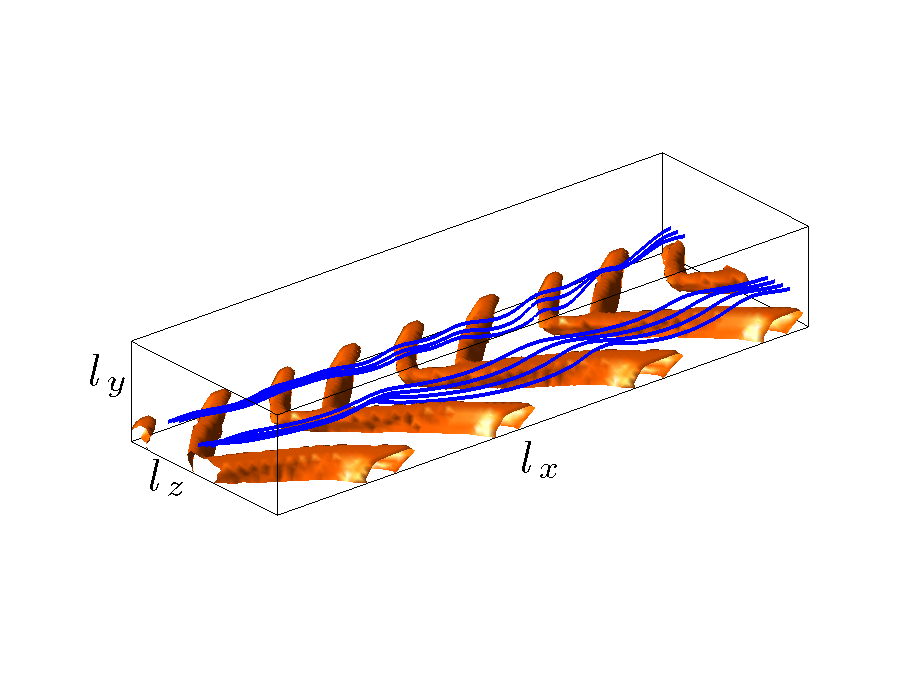
\includegraphics[width=0.5\textwidth]{example2structureherringbone}
     \vspace{-1cm}
      }
    \caption{\label{example2structureNew} THE OPTIMIZED CHANNEL
      STRUCTURE TO PRODUCE ONE BIG AND ONE SMALL VORTEX.}
  \end{figure}
%%%%%%%%%%%%%%%%%%%%%%%%%%%%%%%%%%%%%%%%%%%%%%%

%%%%%%%%%%%%%%%%%%%%%%%%%%%%%%%%%%%%%%%%%%%%%%%
%mixing trajectory
  \begin{figure}
    \centerline{
     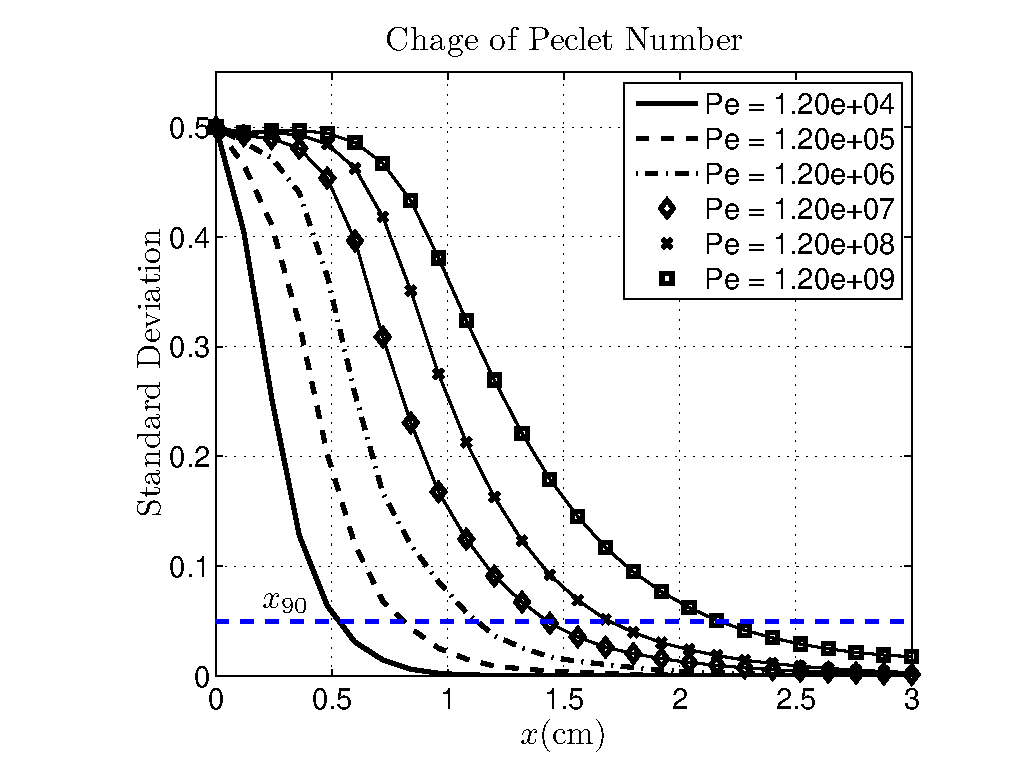
\includegraphics[width=0.45\textwidth]{example2veryPe2}}
     \caption{\label{example2trajectory} MICROFLUIDIC MIXING AS A
       FUNCTION OF CHANNEL LENGTH, FOR VARYING $\text{Pe}$, USING THE
       OPTIMIZED HERRINGBONE STRUCTURED CHANNEL. THE MIXING
       TRAJECTORIES STAYS ALMOST $0.5$ FOR A LONGER DISTANCE WHEN
       $\text{Pe}$ IS LARGE.}
  \end{figure}
%%%%%%%%%%%%%%%%%%%%%%%%%%%%%%%%%%%%%%%%%%%%%%%


%%%%%%%%%%%%%%%%%%%%%%%%%%%%%%%%%%%%%%%%%%%%%%%
% normalized plot
  \begin{figure}
    \begin{center}
     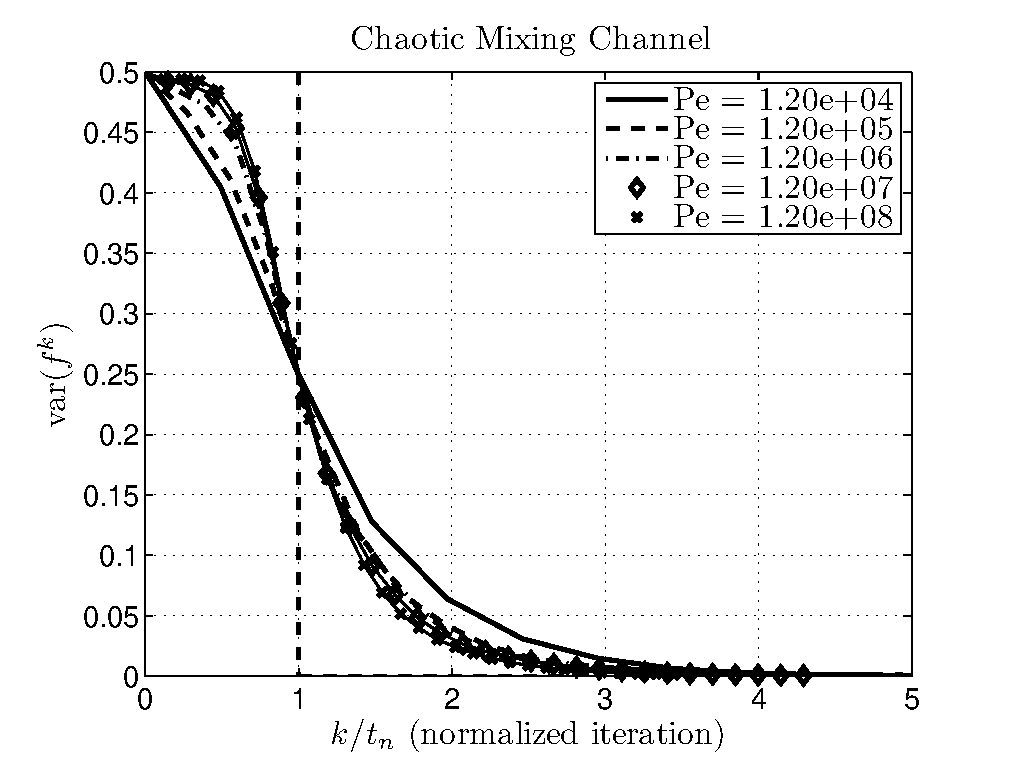
\includegraphics[width=0.4\textwidth]{mixingchannelcutoff}
    \end{center} 
     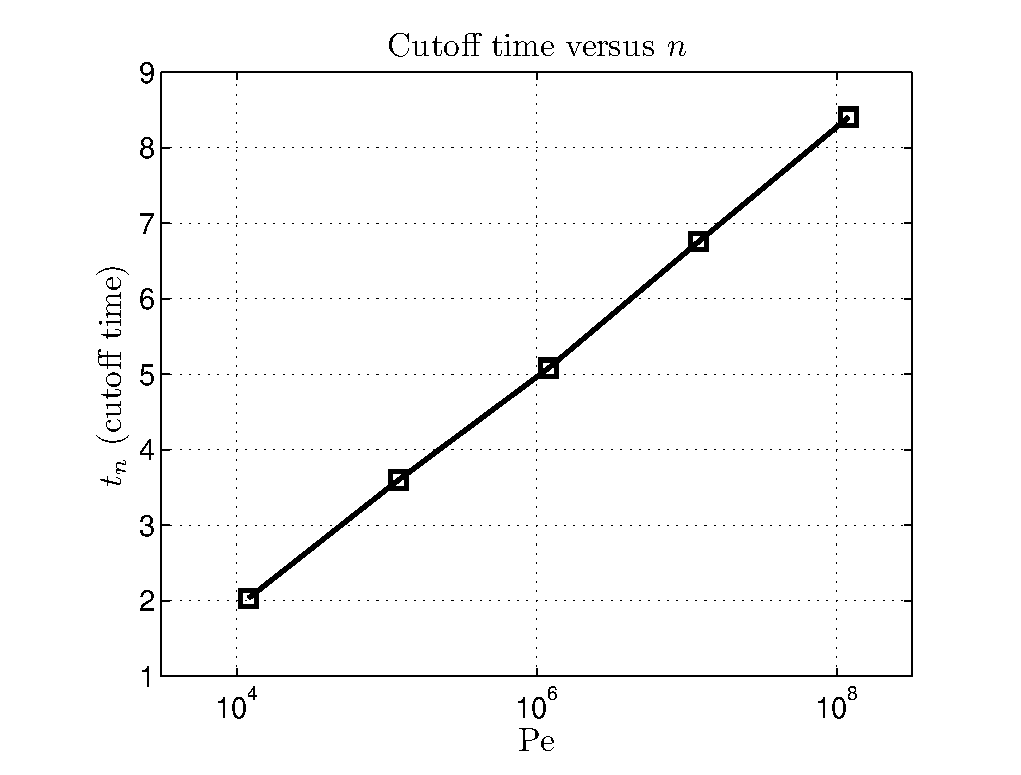
\includegraphics[width=0.23\textwidth]{mixingchannelcutofftimevsPe}
     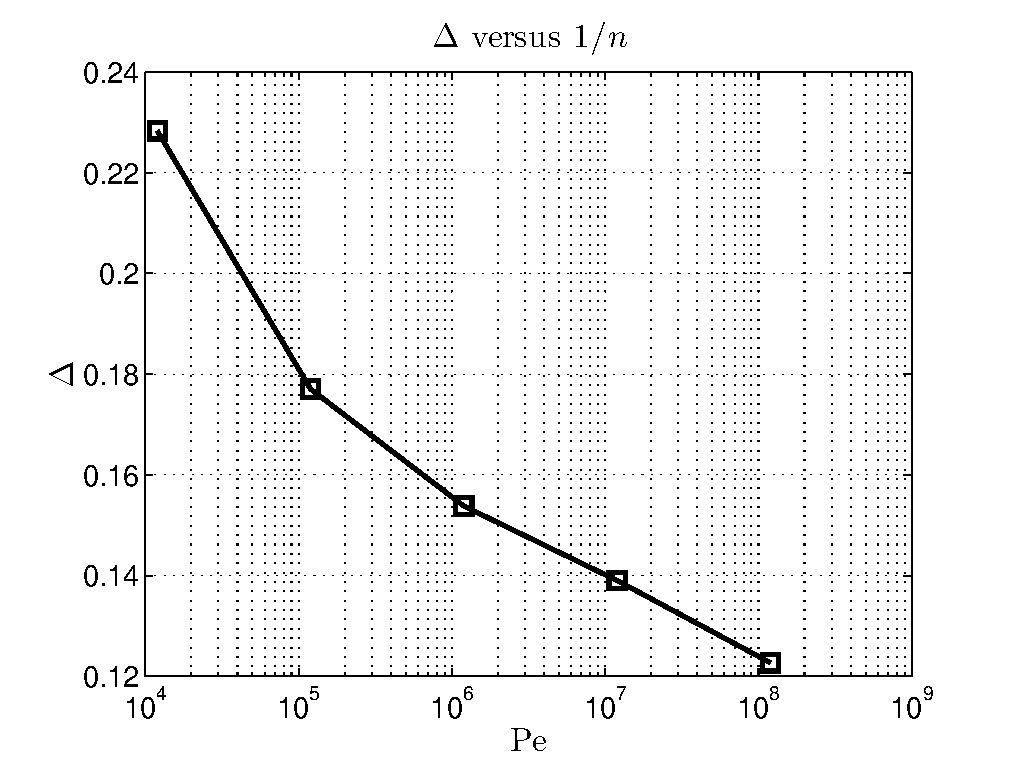
\includegraphics[width=0.23\textwidth]{mixingchannelareavsPe}
    \caption{\label{mixingchannelcutoff} TOP: NORMALIZED TRAJECTORIES
      OF THE MICROFLUIDIC MIXING CHANNEL. BOTTOM LEFT: NEAR LINEAR
      RELATION BETWEEN CUTOFF TIME $t_n$ AND $\text{Pe}$. BOTTOM
      RIGHT: $\Delta_{\hat{B}}^3$ AS A FUNCTION OF $\text{Pe}$. THE
      DECREASE OF $\Delta_{\hat{B}}^3$ WITH $t_n$ SUGGESTS A CUTOFF.}
  \end{figure}
%%%%%%%%%%%%%%%%%%%%%%%%%%%%%%%%%%%%%%%%%%%%%%%

%%%%%%%%%%%%%%%%%%%%%%%%%%%%%%%%%%%%%%%%%%%%%%%
%cross-section simulation 1, for different Pe
  \begin{figure}
    \centerline{
     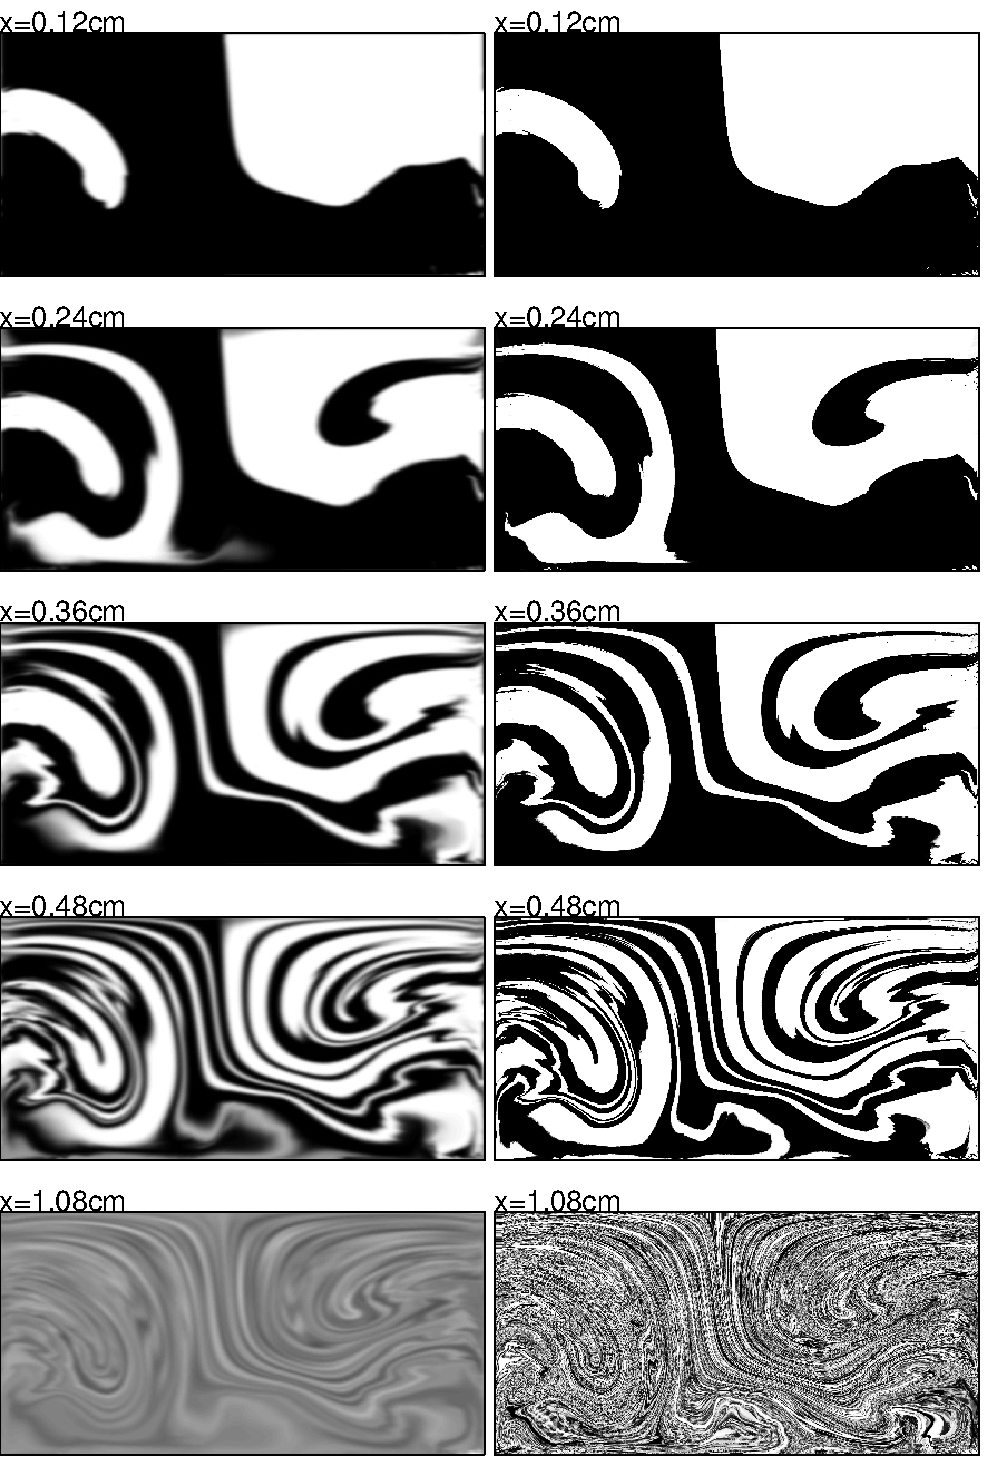
\includegraphics[width=0.4\textwidth]{example2simu2} 
    }
    \caption{\label{example2simu} CHANNEL CROSS-SECTIONS AT THE END OF
      CYCLES 1, 2, 3, 4, 9 (TOP TO BOTTOM) FOR $\text{Pe} =
      1.2\times10^6$ (LEFT) AND $1.2\times10^9$ (RIGHT).}
  \end{figure}
%%%%%%%%%%%%%%%%%%%%%%%%%%%%%%%%%%%%%%%%%%%%%%%





%%%%%%%%%%%%%%%%%%%%%%%%%%%%%%%%%%%%%%%%%%%%%%%%%%%%%%%%%%%%%%%%%%%%%%
\section*{THE SUPER-EXPONENTIAL MIXING CURVE}%%%%%%%%%%%%%%%%%%%%%%%%%
%%%%%%%%%%%%%%%%%%%%%%%%%%%%%%%%%%%%%%%%%%%%%%%%%%%%%%%%%%%%%%%%%%%%%%
In this section we use a simple example to explain why we expect to
see the concave mixing trajectory in the beginning of a chaotic mixing
process. Consider the Baker's map on $T^2$:
\begin{equation*}
     S(x_1,x_2) =
      \begin{cases}
        (2x_1,\frac{1}{2}x_2) \text{ mod } 1,
        & \text{if } 0 \le x_1 < \frac{1}{2} \\
        (2x_1,\frac{1}{2}(x_2+1)) \text{ mod } 1,
        & \text{if } \frac{1}{2} \le x_1 < 1
      \end{cases}
\end{equation*}
with initial condition $f^0(x)= \sqrt{\pi} \cos(2 \pi x_2)$. The
action of the Koopman operator on $f^0(x)$ is very simple: it doubles
the frequency of the cosine wave at each iteration, as shown in
Figure~\ref{bakersmapsimu}. We further apply a diffusion operator with
diffusivity $D$ after every iteration to make the process
diffusive. Just like in the mixing channel problem, we want to know
how the variance changes with iteration number $k$. This problem is
analytically solvable:
\begin{align*}
      f^k(x) &= \sqrt{\pi} e^{-4 \pi^2 D 2 ^{2 k}}\cos(2 \pi 2^k x_2)
      \text{ for } k = 1,2,\ldots
\end{align*}
and the variance of $(f^k(x))$ is $\text{var}(f^k(x)) = e^{-8 \pi^2 D
  2^{2 k}}$, a doubly exponential function of $k$. We plot
$\text{var}(f^k(x))$ in Figure~\ref{bakersmapcutoff} with different
$D$ values. This figure shows that the set of trajectories presents a
cutoff with cutoff time $t_n \sim -\log(D)$. The trajectories we see
in the mixing channel simulation have the same tendency as the Baker's
Map simulation. In the next section we numerically simulate another
discrete map, the Standard Map, to provide the additional numerical
evidence of the cutoff in chaotic maps.


\begin{figure}
    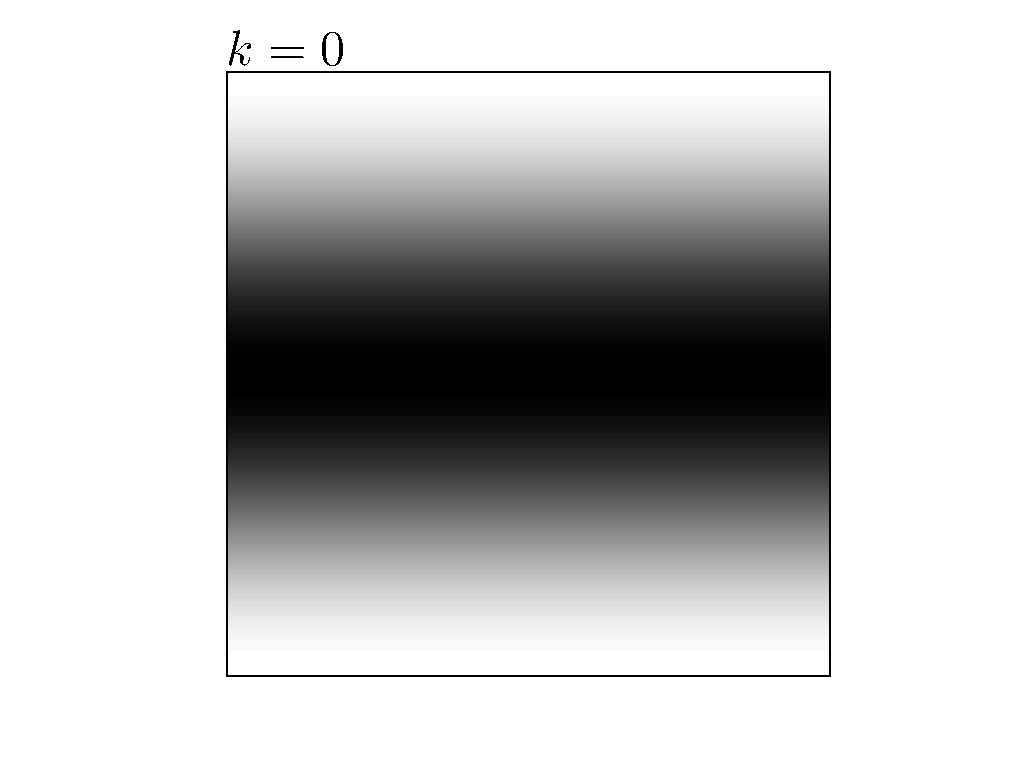
\includegraphics[width=0.15\textwidth,trim=2.5cm 0cm 2.5cm 0cm,clip]{bakers1}
    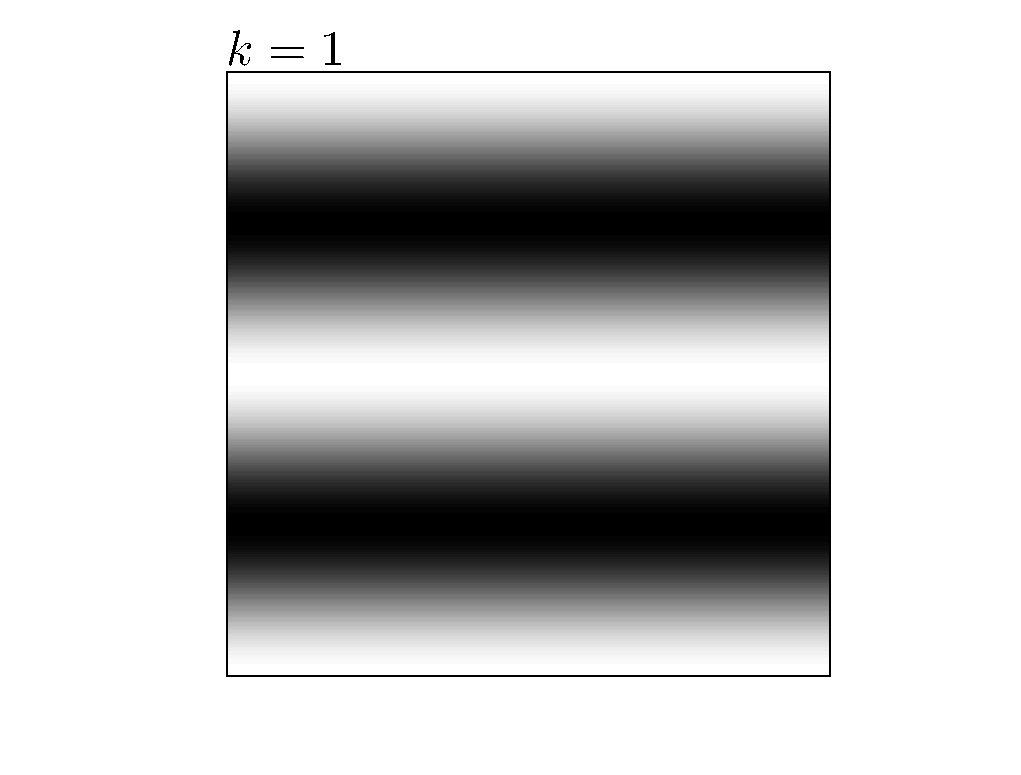
\includegraphics[width=0.15\textwidth,trim=2.5cm 0cm 2.5cm 0cm,clip]{bakers2}
    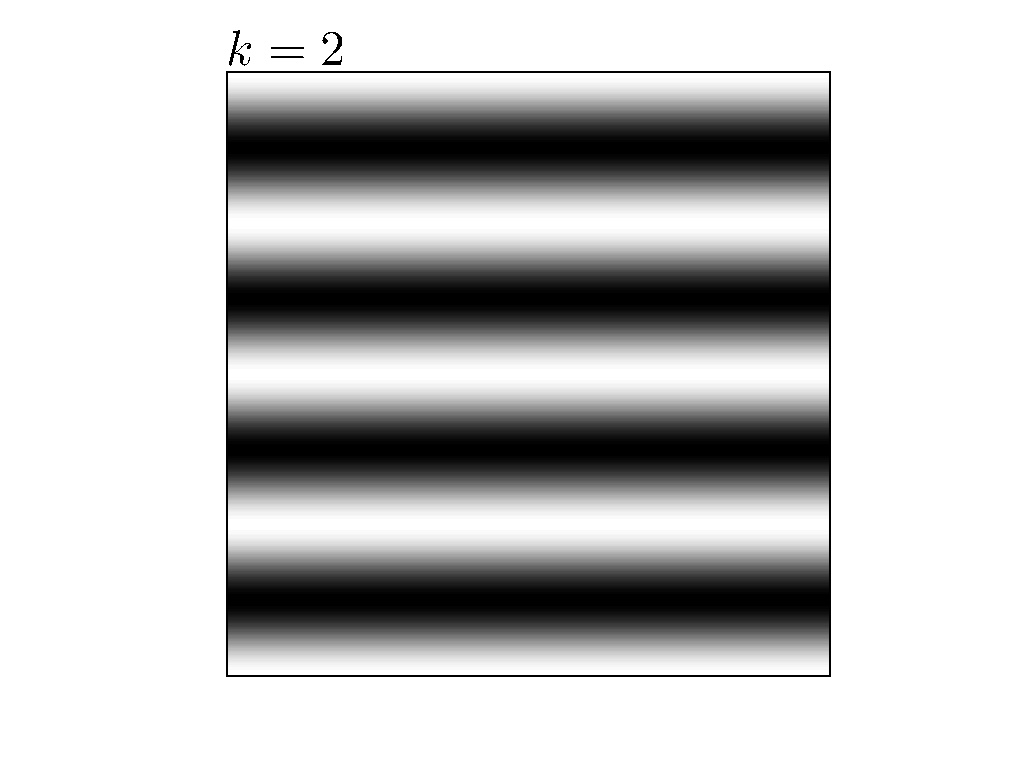
\includegraphics[width=0.15\textwidth,trim=2.5cm 0cm 2.5cm 0cm,clip]{bakers3}
     \caption{\label{bakersmapsimu} THE FIRST THREE ITERATIONS OF A
       FUNCTION $f^0=\cos(2 \pi x_2)$ ADVECTED BY THE BAKER'S MAP. IT
       SIMPLY DOUBLES THE FREQUENCY OF THE COSINE FUNCTION IN THE $x_2$
       DIRECTION.}
\end{figure}



\begin{figure}
    \begin{center}
      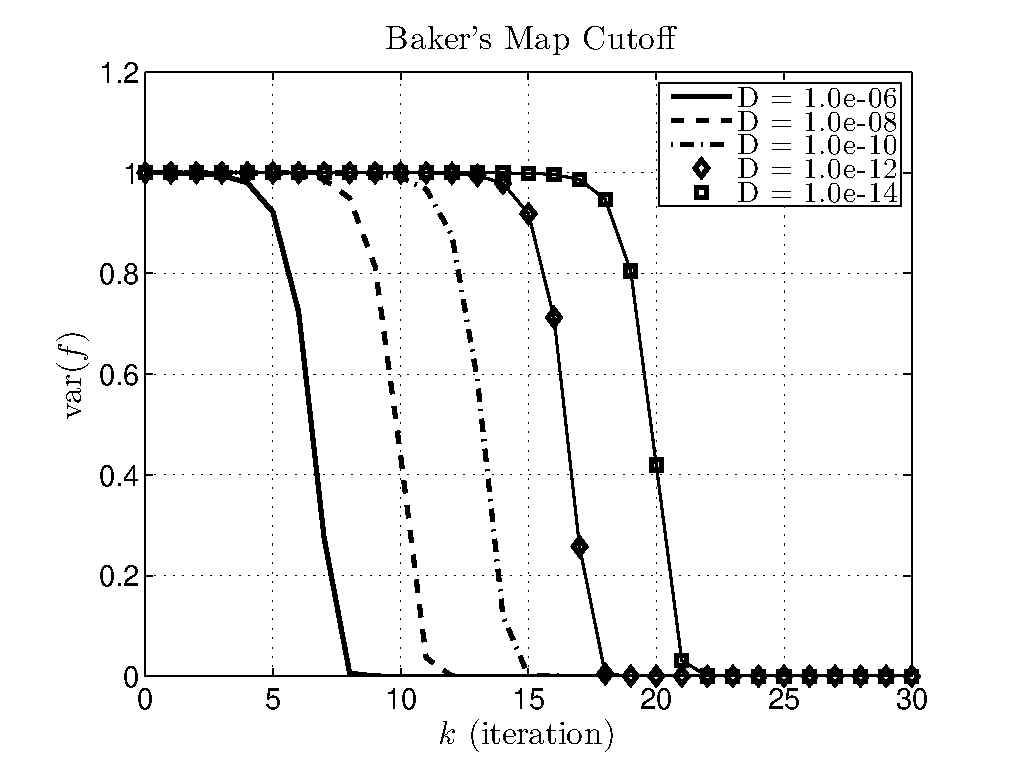
\includegraphics[width=0.45\textwidth]{bakersmapcutoff}
    \end{center}
     \caption{\label{bakersmapcutoff} VARIANCE EVOLUTION OF A FUNCTION
       ADVECTED BY THE BAKER'S MAP, SHOWING CUTOFF.}
\end{figure}


%%%%%%%%%%%%%%%%%%%%%%%%%%%%%%%%%%%%%%%%%%%%%%%%%%%%%%%%%%%%%%%%%%%%%%
\section*{STANDARD MAP SIMULATION}%%%%%%%%%%%%%%%%%%%%%%%%%%%%%%%%%%%%
%%%%%%%%%%%%%%%%%%%%%%%%%%%%%%%%%%%%%%%%%%%%%%%%%%%%%%%%%%%%%%%%%%%%%%


We study the Standard Map on $T^2$:
   \begin{align}
   \label{Standardmap}
               x_1' &= x_1+x_2 +\epsilon \sin{2 \pi x_1}  \ (\mbox{mod } 1), \nonumber\\
               x_2' &=  x_2 +\epsilon \sin{2 \pi x_1}     \ (\mbox{mod } 1).
   \end{align}
This map is known to be chaotic for certain values of
$\epsilon$. Various studies of how a point is advected by the map can
be found, for example, in~\cite{Ott2002}. Here we mainly focus on how
a scalar function is evolved by the map with additional small
diffusion. Because this map is volume preserving, its invariant
measure is uniform. We always scale the mean and standard deviations
of $f^0$ to be $1$. The Standard Map is known to have some non-chaotic
region when $\epsilon$ is not zero, so the distance $d$ converges to a
value $m \neq 0$, which is why Definition~\ref{cutoffdefinitionn} of
cutoff is slightly modified from that in~\cite{Diaconis2005}.

The evolution of the variance of $f^k_n$ with $n$ ranging from
$2500^2$ to $80000^2$ using $B_n$ and $\bar{B}_n$ as the Koopman
operators are shown in the left of Figures~\ref{standardmapun}
and~\ref{smoothingstandardmapun}. The tendency is clear: as $n$
becomes larger, the variance stays high ($M_B=M_{\bar{B}}=1$) for more
iterations and then drops rapidly to $m_{B} = 0.4521$ and
$m_{\bar{B}}=0.4498$, respectively---they do not drop to zero because
there are unmixed ``islands''. The rapid dropping region also becomes
slightly longer when $n$ increases. To see whether this evolution
presents a cutoff, we let $t_n$ be the time where each trajectory
passes through $(M_{\star}+m_{\star})/2$, where $\star=\{B,\bar{B}\}$,
and normalize all the trajectories by rescaling $t_n$ to $1$. The
results are plotted in the right of Figures~\ref{standardmapun}
and~\ref{smoothingstandardmapun}. Although the normalized trajectories
are very similar, one can still see that when $n$ gets larger, the
trajectory becomes sharper. In the upper plot of
Figure~\ref{cutofftimeandarea} we plot $t_n$ versus $1/n$ on a
logarithmic scale and we see two straight lines. Note that for both
cases, we have $D\sim O(1/n)$. Hence this plot shows that the cutoff
time is inversely proportional $\log(D)$. Just like we did in the
mixing channel trajectories, we plot $\Delta^3_B$ and
$\Delta^3_{\bar{B}}$ versus $t_n$ in the right of
Figure~\ref{cutofftimeandarea}, showing that when $t_n$ increases,
both $\Delta_{B}^3$ and $\Delta_{\bar{B}}^3$ decay slightly
sub-linearly, but clearly as $n$ grows, $\Delta^3_{B}$ and
$\Delta^3_{\bar{B}}$ decrease, which strongly suggests that both
sequences of Markov Chains present cutoffs.

%$\{B_n, g_n(\cos(2\pi x_2)) \}$ and $\{\bar{B}_n, g_n(\cos(2\pi x_2)) \}$ present cutoffs.


%%%%%%%%%%%%%%%%%%%%%%%%%%%%%%%%%%%%%%%%%%%%%%%%%%%%%%%%%%%%%%%%%%%%%%
%%%%%%%%%%%%%%%% begin figure %%%%%%%%%%%%%%%%%%%
\begin{figure}
      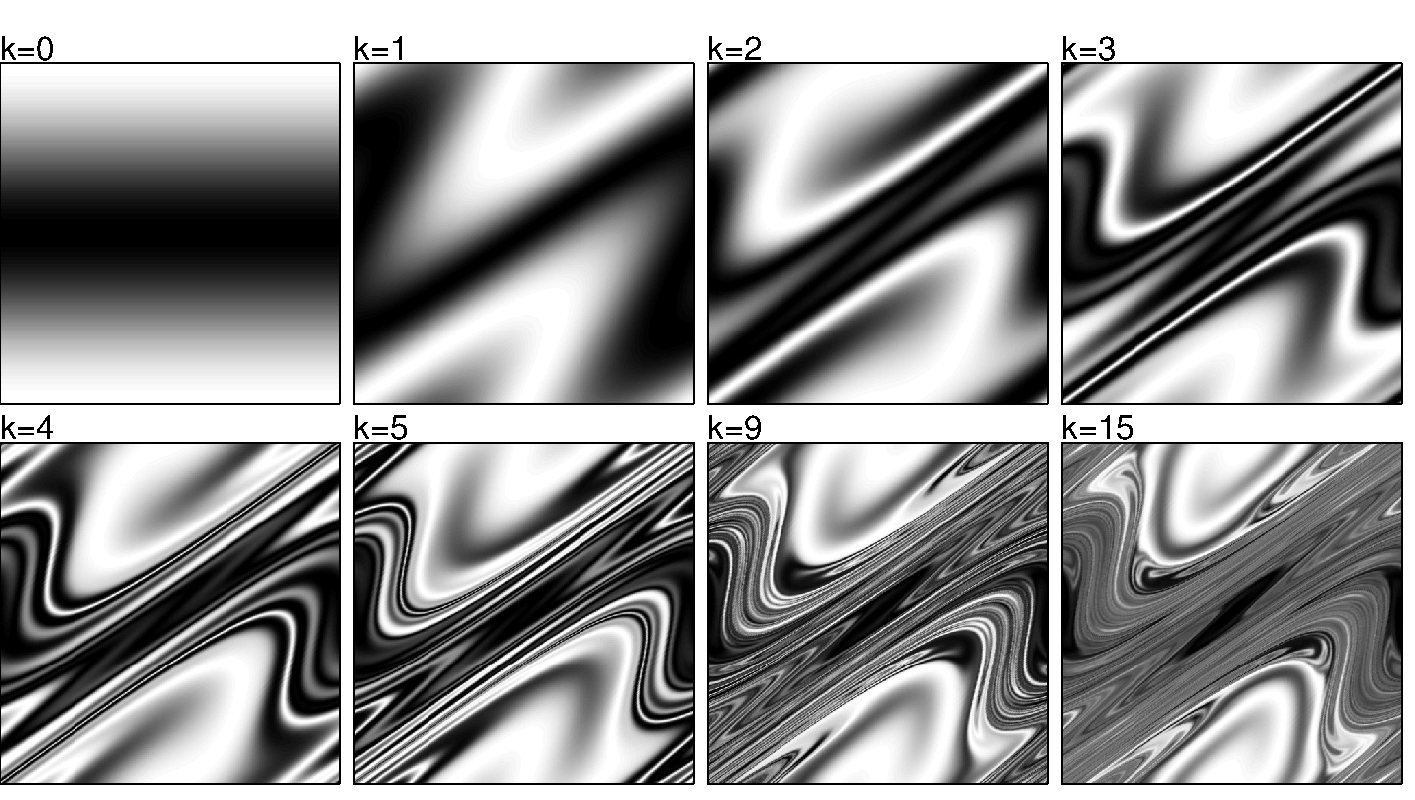
\includegraphics[width=0.45\textwidth]{standardmapevolve}
     \caption{\label{standardmapevolve} THE FIRST EIGHT ITERATIONS OF
       $f^k_n$ WHEN $f^0 = \cos(2\pi x_2)$ IS ADVECTED BY THE STANDARD
       MAP WTIH $\epsilon=0.3$ AND $n = 500$.}
\end{figure}
%%%%%%%%%%%%%%%% end figure %%%%%%%%%%%%%%%%%%%

%%%%%%%%%%%%%%%%%%%%%%%%%%%%%%%%%%%%%%%%%%%%%%%%%%%%%%%%%%%%%%%%%%%%%%
%%%%%%%%%%%%%%%% begin figure %%%%%%%%%%%%%%%%%%%
\begin{figure}
      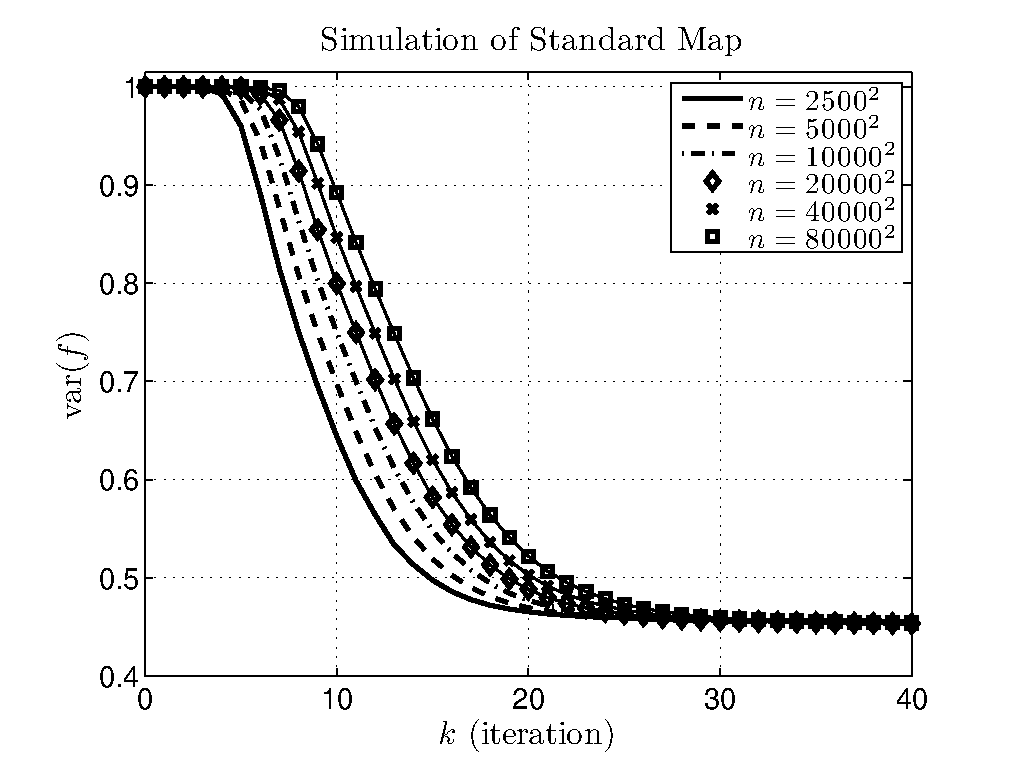
\includegraphics[width=0.45\textwidth]{standardmapcutoff}
      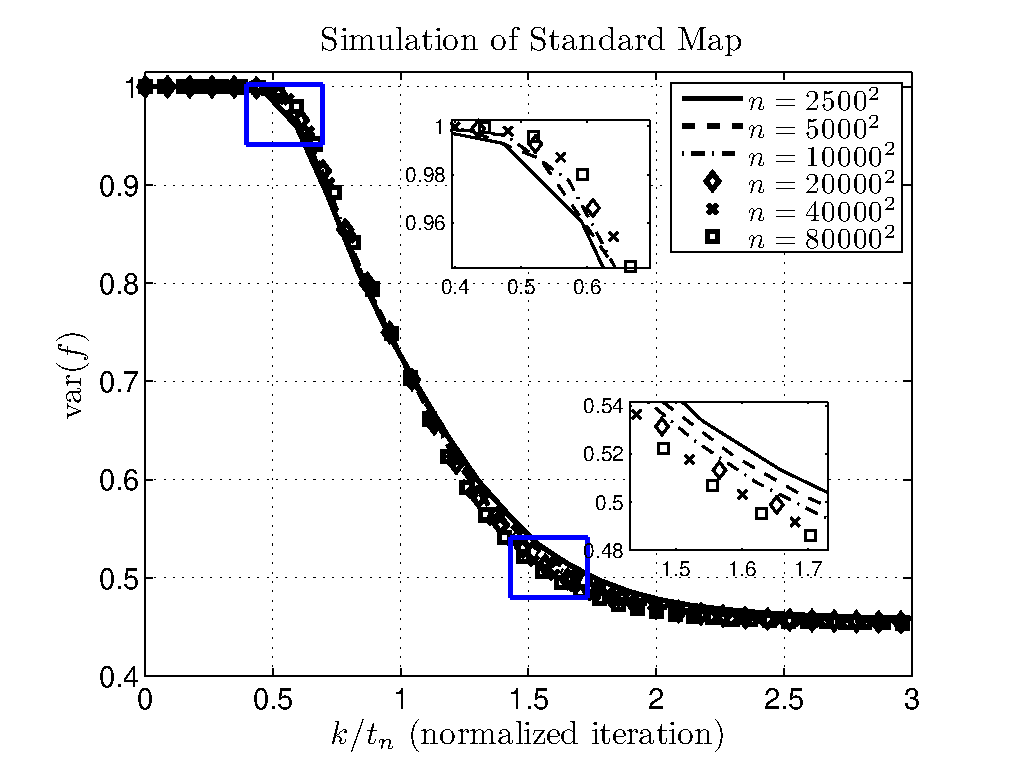
\includegraphics[width=0.45\textwidth]{standardmapcutoffn}
    \caption{\label{standardmapun} TOP: VARIANCE OF $f_n^k$ VERSUS
      ITERATION NUMBER FOR THE STANDARD MAP. WE USE $\epsilon=0.3$,
      $f^0=\cos(2 \pi x_2)$, AND NUMBER OF GRID CELLS $n$ VARIES FROM
      $2500^2$ TO $80000^2$. BOTTOM: RESCALED VERSION OF THE TOP PLOT,
      SO THAT ALL TRAJECTORIES PASS THROUGH THE POINT
      $(1,0.7260)$. THE TWO SMALL PLOTS SHOW DETAILED VIEWS OF THE
      CORNERS.}
\end{figure}
%%%%%%%%%%%%%%%% end figure %%%%%%%%%%%%%%%%%%%
%%%%%%%%%%%%%%%%%%%%%%%%%%%%%%%%%%%%%%%%%%%%%%%%%%%%%%%%%%%%%%%%%%%%%%

\begin{figure}
      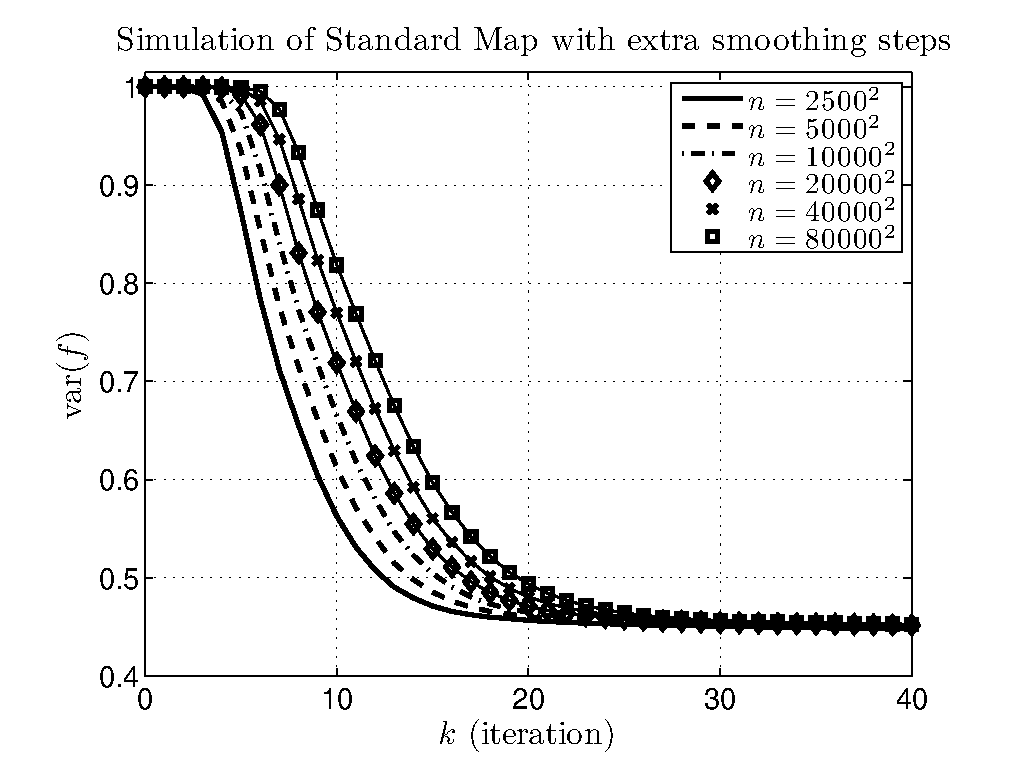
\includegraphics[width=0.45\textwidth]{standardmapcutoffwithsmoothing}
      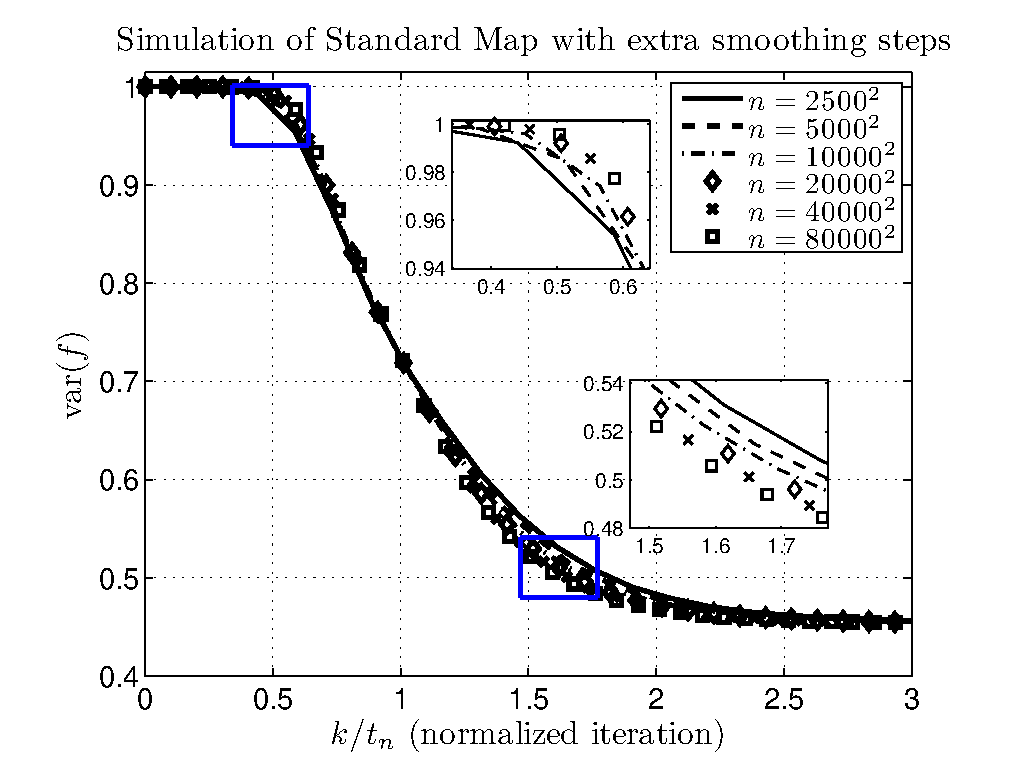
\includegraphics[width=0.45\textwidth]{standardmapcutoffwithsmoothingn}
     \caption{\label{smoothingstandardmapun} TOP: VARIANCE OF $f_n^k$
       VERSUS ITERATION NUMBER FOR THE STANDARD MAP SIMULATION WHEN A
       SMOOTHING STEP IS ADDED AFTER EACH ITERATION. WE USE
       $\epsilon=0.3$, $f^0=\cos(2 \pi x_2)$, AND NUMBER OF GRID CELLS
       $n$ VARIES FROM $2500^2$ TO $80000^2$. BOTTOM: RESCALED VERSION
       OF THE TOP PLOT, SO THAT ALL TRAJECTORIES PASS THROUGH THE
       POINT $(1,0.7260)$. THE TWO SMALL PLOTS SHOW DETAILED VIEWS OF
       THE CORNERS.}
\end{figure}


%%%%%%%%%%%%%%%%%%%%%%%%%%%%%%%%%%%%%%%%%%%%%%%%%%%%%%%%%%%%%%%%%%%%%%
%%%%%%%%%%%%%%%% begin figure %%%%%%%%%%%%%%%%%%%
\begin{figure}
   \label{cutofftime}
      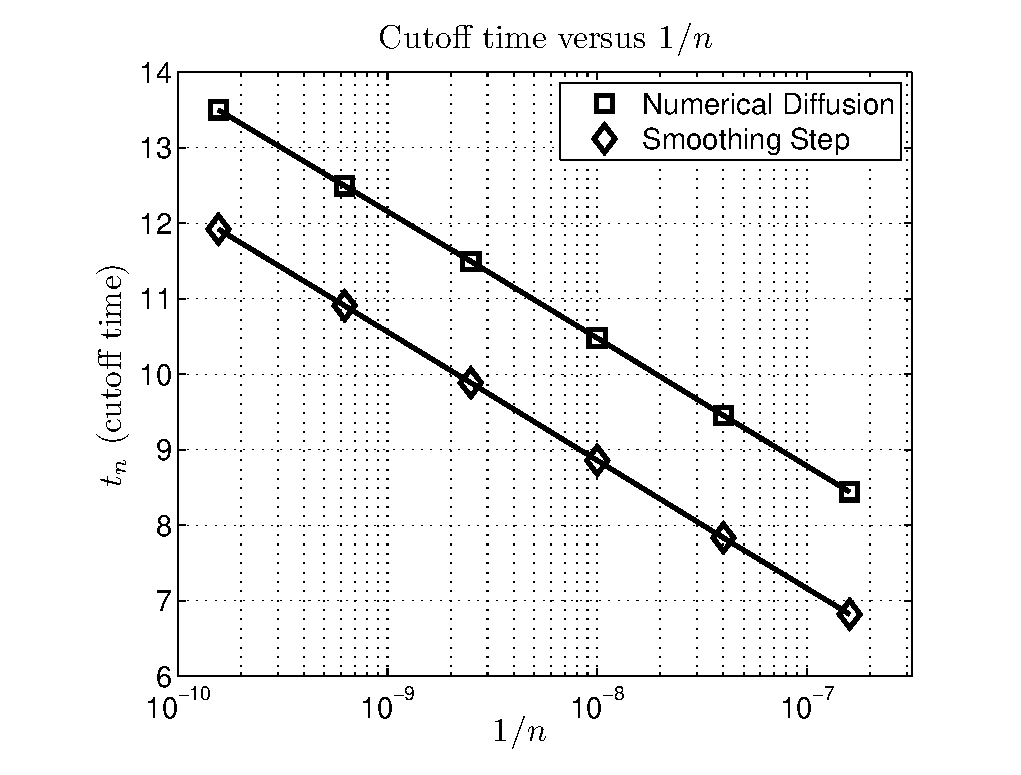
\includegraphics[width=0.45\textwidth]{cutofftimevsD}
      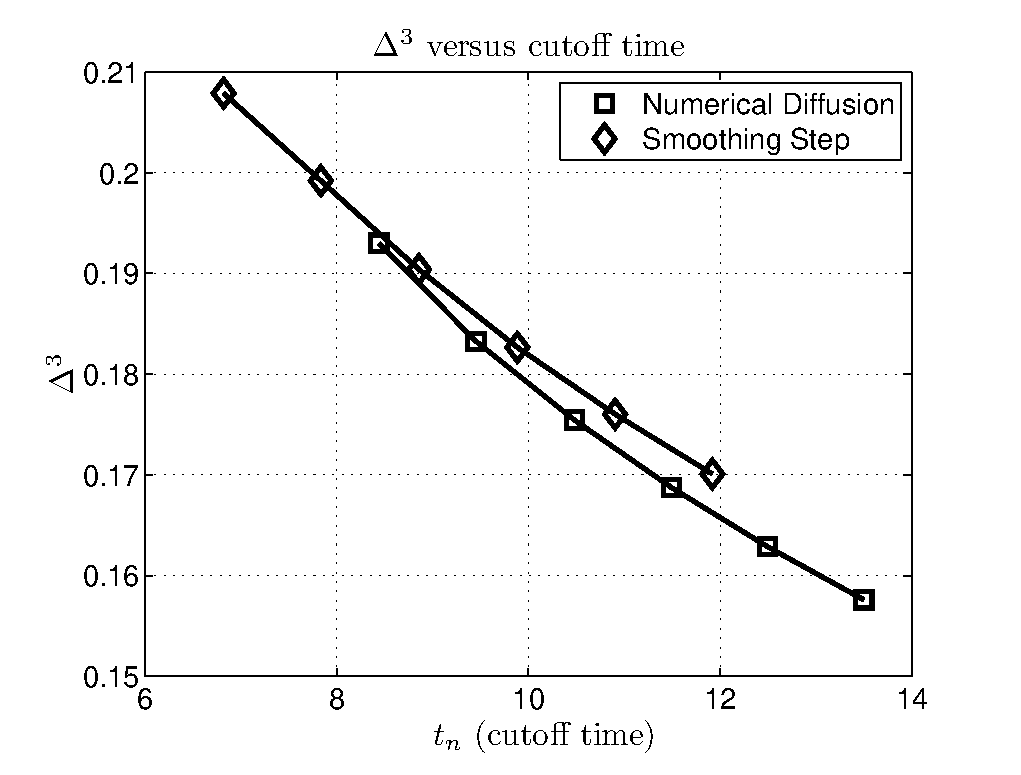
\includegraphics[width=0.45\textwidth]{areavscutofftime}
     \caption{\label{cutofftimeandarea} TOP: CUTOFF TIME $t_n$ RELATED
       TO $1/n$ ON A LOGARITHMIC SCALE. SINCE WE HAVE $D \sim O(1/n)$
       FOR OUR SIMULATION STRATEGY, ONE CAN CONCLUDE THAT $t_n$ IS
       INVERSELY PROPORTIONAL TO $\log(D)$. BOTTOM: CONVERGENCE OF
       NORMALIZED TRAJECTORIES TO THEIR LIMITS. $\Delta^3$ IS DEFINED
       IN EQUATION~(\ref{trajdistance}). BOTH CURVES PREDICT THAT WHEN
       $t_n$ IS VERY LARGE, $\Delta^3$ GOES DOWN, AND THE NORMALIZED
       TRAJECTORY WOULD LIKELY LIMIT TO A STEP FUNCTION.}
\end{figure}
%%%%%%%%%%%%%%%% end figure %%%%%%%%%%%%%%%%%%%
%%%%%%%%%%%%%%%%%%%%%%%%%%%%%%%%%%%%%%%%%%%%%%%%%%%%%%%%%%%%%%%%%%%%%%








%%%%%%%%%%%%%%%%%%%%%%%%%%%%%%%%%%%%%%%%%%%%%%%%%%%%%%%%%%%%%%%%%%%%%%
\section*{CONCLUSION}
We provide numerical evidence that mixing processes in a number of
fluid and chaotic map systems present cutoffs in the sense of finite
Markov Chains, in the limit of small diffusion. This means that as the
diffusion tends to zero, the time over which the variance of an
advected scalar function decreases significantly tends to zero,
relative to the onset time of the decrease.
%%%%%%%%%%%%%%%%%%%%%%%%%%%%%%%%%%%%%%%%%%%%%%%%%%%%%%%%%%%%%%%%%%%%%%
\bibliographystyle{asmems4}
\bibliography{../bib/mixingbib}



\end{document}
